% Appendices A-F of the ARC Prize 2026 (ARC-AGI-2) solution writeup, team okiek.
% Build:  tectonic solution_writeup_appendix.tex    (or: latexmk -xelatex / -lualatex / -pdf)
% The figure is read from figures/ next to this file.
\documentclass[10pt]{article}

\usepackage[letterpaper,margin=1in,headheight=14pt]{geometry}
\usepackage{iftex}
\usepackage{amsmath}
\ifPDFTeX
  \usepackage[T1]{fontenc}
  \usepackage[utf8]{inputenc}
  \usepackage[lining]{libertinus}
  \usepackage{libertinust1math}
  \newcommand{\appminus}{\textminus}
\else
  \usepackage{unicode-math}
  \setmainfont{LibertinusSerif}[Extension=.otf, UprightFont=*-Regular, BoldFont=*-Bold,
    ItalicFont=*-Italic, BoldItalicFont=*-BoldItalic, Numbers=Lining]
  \setmonofont{LibertinusMono}[Extension=.otf, UprightFont=*-Regular, Scale=MatchLowercase, WordSpace={1,0,0}]
  \setmathfont{LibertinusMath-Regular.otf}
  \newcommand{\appminus}{\symbol{"2212}}
\fi

\usepackage{xcolor}
\definecolor{ink}{RGB}{33,37,41}
\definecolor{muted}{RGB}{95,99,104}
\definecolor{accent}{RGB}{31,78,140}
\usepackage{graphicx}
\graphicspath{{figures/}}
\usepackage{booktabs}
\usepackage{tabularx}
\usepackage{array}
\usepackage{float}
\usepackage{enumitem}
\setlist{topsep=2pt, itemsep=1pt, parsep=0pt, partopsep=0pt}
\setlist[itemize]{leftmargin=1.3em, label={\color{muted}\textbullet}}
\usepackage[font=small, labelfont={bf,color=accent}, skip=5pt]{caption}
\usepackage{titlesec}
\usepackage{fancyhdr}
\usepackage{microtype}
\usepackage[colorlinks=true, linkcolor=accent, urlcolor=accent, citecolor=accent,
  pdftitle={Appendices: Throughput is accuracy (ARC Prize 2026, team okiek)},
  pdfauthor={Team okiek}, pdfsubject={ARC Prize 2026, ARC-AGI-2 solution writeup}]{hyperref}

% Lettered sections read "Appendix A  Compression recipe"; run-in bold paragraph heads.
\titleformat{\section}{\normalfont\Large\bfseries\color{ink}}{\color{accent}Appendix~\thesection}{0.6em}{}
\titlespacing*{\section}{0pt}{3.2ex plus .6ex minus .2ex}{1.4ex plus .2ex}
\titleformat{\paragraph}[runin]{\normalfont\normalsize\bfseries\color{ink}}{}{0pt}{}
\titlespacing*{\paragraph}{0pt}{1.3ex plus .4ex minus .2ex}{0.55em}
\setlength{\parindent}{0pt}
\setlength{\parskip}{3pt plus 1pt}
\renewcommand{\arraystretch}{1.18}
\newcommand{\Dpm}[3]{#1\,[#2,\,#3]}          % difference with its interval
\newcommand{\mn}{\appminus}                     % text minus sign
\newcolumntype{L}{>{\raggedright\arraybackslash}X}

\pagestyle{fancy}
\fancyhf{}
\fancyhead[L]{\small\color{muted}\itshape Throughput is accuracy: appendices}
\fancyhead[R]{\small\color{muted}\itshape ARC Prize 2026, team okiek}
\fancyfoot[C]{\small\color{muted}\thepage}
\renewcommand{\headrulewidth}{0.3pt}
\fancypagestyle{plain}{\fancyhf{}\fancyfoot[C]{\small\color{muted}\thepage}\renewcommand{\headrulewidth}{0pt}}

\begin{document}
\thispagestyle{plain}
\color{ink}

\begin{center}
  {\small\scshape\color{muted} Supplementary material to the solution writeup}\\[6pt]
  {\LARGE\bfseries Appendices A--F}\\[8pt]
  {\large Throughput is accuracy: a verified program-writing agent\\ on a compressed 125B MoE at 1,100 tokens/s on four L4s}\\[8pt]
  {\normalsize Team okiek \quad\textcolor{muted}{|}\quad ARC Prize 2026, ARC-AGI-2}
\end{center}
\vspace{4pt}

These appendices accompany our solution writeup. They hold the recipes, hyperparameters and negative results behind
its main text: compression (\hyperref[app:compression]{Appendix~A}), reinforcement learning on the quantization scales
(\hyperref[app:rl]{B}), the draft head (\hyperref[app:draft]{C}), the agent harness (\hyperref[app:harness]{D}),
scheduling, the deadline and answer selection (\hyperref[app:scheduling]{E}), and the serving engine
(\hyperref[app:engine]{F}).

\paragraph{Conventions.} Scores and differences are percentage points on the 120 public ARC-AGI-2 evaluation tasks,
our local set; brackets give intervals. ``pass@2 at 100k tokens'' means a budget of 100k generated tokens per test
input. ×8 and ×79 denote offline pools of 8 and 79 sessions per task, which carry about ±3.5 and ±0.8 points of noise.
REPL is the program-writing agent, and FP8 is the unpruned model at FP8.

\appendix
\counterwithin{table}{section}
\counterwithin{figure}{section}

% ---------------------------------------------------------------------------------------------------------------
\section{Compression recipe}\label{app:compression}

\paragraph{Calibration.} The FP8 model's own attempts on ARC-AGI-2 training tasks: 1,040 sequences on 480 tasks (688 on
320 random tasks at a 64k cap, 352 on 160 harder tasks at 96k), with 48 tasks held out. Teacher-forced replay records
routing over 12.6M tokens per layer.

\paragraph{Keep score.} Each expert $e$ is scored by
\begin{equation*}
  \mathrm{score}(e) \;=\; \sum_{t} g_{t,e}\,\lVert y_{t,e}\rVert_2 \;+\; 0.5\, m^{\mathrm{call}}_{e} \;+\; 0.25\, m^{\mathrm{resp}}_{e},
\end{equation*}
where $g_{t,e}$ is the gate weight and $y_{t,e}$ the expert's output on token $t$, and $m^{\mathrm{call}}_{e}$ and
$m^{\mathrm{resp}}_{e}$ are its routing mass on tool-call and tool-response tokens. Each of the three terms is normalized.
\begin{itemize}
  \item $K = 320$ in every layer, including the MTP layer; the top 10 are renormalized over the kept experts.
  \item A plain usage cut keeps the share of held-out routing weight in Table~\ref{tab:coverage}.
  \item At $K = 256$, also protecting the experts that carry 90\% of header routing raised header coverage from 0.76
        to 0.94, with 0 format errors in 90 sessions.
  \item Every keep set gets at least 30 REPL sessions of format checks.
\end{itemize}

\begin{table}[H]
  \centering\small
  \caption{Held-out routing weight kept by a plain usage cut, by experts kept per layer ($K$ of 512).}
  \label{tab:coverage}
  \begin{tabular}{@{}lrrrrrr@{}}
    \toprule
    Experts kept, $K$ & 448 & 384 & 320 & 256 & 192 & 128 \\
    \midrule
    Routing weight kept & 99.3\% & 97.5\% & 94.3\% & 89.4\% & 82.1\% & 71.4\% \\
    \bottomrule
  \end{tabular}
\end{table}

\paragraph{GPTQ.}
\begin{itemize}
  \item Group size 128, asymmetric (fp16 scale, uint8 zero).
  \item Per-group MSE clip search over 10 ratios, from 1.0 to 0.55; activation ordering; damping
        $\operatorname{mean}(\operatorname{diag} H)\cdot(0.01 + 4/n)$ for $n$ calibration rows.
  \item Hessians come from router-weighted inputs under the pruned routing. Gate and up are quantized jointly; the
        down projection's Hessian uses the quantized activations.
\end{itemize}

\paragraph{Kernels.} 4-bit experts run on Marlin. 3-bit experts run on our Triton GEMM (planar layout, \texttt{lop3}
dequantization), at 374\,µs per layer for 64 rows against 476\,µs for Marlin 4-bit. The two groups run concurrently:
725.6\,MB per layer, 8.7\,GB per GPU.

\paragraph{Dense layers.}
\begin{itemize}
  \item Online per-channel FP8 W8A8 for the Gated DeltaNet projections, shared experts and LM head. REPL tests read
        +5.4 / +4.4 at 40 / 80k tokens (intervals span 0), and it frees memory for 29--31\% more KV.
  \item The other dense weights stay BF16.
\end{itemize}

\paragraph{Cost against FP8.} Table~\ref{tab:cost} compares builds by REPL pass@2 at 80k tokens.

\begin{table}[H]
  \centering\small
  \caption{Cost of each build against the FP8 model (REPL pass@2 at 80k tokens).}
  \label{tab:cost}
  \begin{tabular}{@{}lr@{}}
    \toprule
    Build & $\Delta$ (points) \\
    \midrule
    320 experts, all 4-bit & \mn5.0 \\
    \textbf{Shipped: 320 experts, 160 at 4-bit and 160 at 3-bit} & \textbf{\mn5.9} \\
    384 experts, FP8 (pruning only) & \mn6.5 \\
    512 experts, 3-bit (quantization only) & \mn6.6 \\
    384 experts, 3-bit & \mn8.3 \\
    256 experts, 3-bit & \mn12.1 \\
    \bottomrule
  \end{tabular}
\end{table}

% ---------------------------------------------------------------------------------------------------------------
\section{RL recipe}\label{app:rl}

\paragraph{Parameters.} A log-offset $t$ on every per-group scale of the kept experts ($s = s_0\, e^{t}$, 589.8M),
plus the kept router rows (39.3M). Everything else is frozen.

\paragraph{Gradient path.}
\begin{itemize}
  \item A plain-PyTorch model: Gated DeltaNet through fla, sparse attention through flex attention with no-grad block
        selection, plus hyper-connections and per-layer embeddings. It matches the reference at logit KL
        $1.5\times10^{-4}$.
  \item A custom autograd function rebuilds $W = s\,(q - z)$ from the packed codes, so
        $\partial L/\partial s = \sum_{\text{group}} \partial L/\partial W \odot (q - z)$.
  \item About 118\,GB peak at 32k tokens.
\end{itemize}

\paragraph{Objective.} REINFORCE with a leave-one-out baseline: $A_i = R_i - \sum_{j \ne i} R_j / (k-1)$ over the
task's $k$ samples, with no std scaling. Flat groups, groups smaller than 4 and zero-advantage samples are dropped.
For the $n$ sequences of a step, the loss is
\begin{equation*}
  \mathcal{L} \;=\; -\frac{1}{n \cdot 16{,}384} \sum_{i=1}^{n} A_i \sum_{t} \log \pi(y_{i,t}),
  \qquad A_i \text{ clipped to } [-2,\, 2].
\end{equation*}
One on-policy pass per round. No KL, PPO clip, entropy bonus, weight decay or gradient clipping.

\begin{table}[H]
  \centering\small
  \caption{RL settings.}
  \label{tab:rl}
  \begin{tabularx}{\linewidth}{@{}>{\bfseries}p{2.9cm}L@{}}
    \toprule
    \multicolumn{1}{@{}l}{Setting} & Value \\
    \midrule
    Optimizer & Adam, $\beta = (0.9,\, 0.99)$, $\epsilon = 10^{-10}$, fp32 master weights \\
    Learning rates & scales $3\times10^{-4}$, router $1.5\times10^{-5}$; 3 warm-up steps, then cosine \\
    Batch and steps & 64 sequences per step; 21, 32 and 30 steps in the shipped rounds \\
    Rollouts & shipped harness; $T = 1.0$, top-$p$ 0.95, top-$k$ 20; about 8 per task \\
    Masking & only sampled spans trained; tool output, nudges and forced answers masked; cut at 32,768 tokens \\
    Rollout servers & vLLM with BF16-dequantized copies of the same codes and the current router; trainer--server
                      log-prob gap 0.053 nats per token \\
    \bottomrule
  \end{tabularx}
\end{table}

\paragraph{Data.}
\begin{itemize}
  \item Only 124 of 948 training tasks gave mixed reward groups: the model already verified 99.0\% of sessions.
  \item So we added leave-one-pair-out variants, in which one demonstration becomes the test.
  \item Later rounds added ARC-AGI-1 tasks and RE-ARC-derived tasks: fresh instances, the hardest decile, and rule
        compositions.
\end{itemize}

\paragraph{Rewards.} The first round-1 reward led to abstention; round 1 shipped with the corrected one
(Table~\ref{tab:reward}).

\begin{table}[H]
  \centering\small
  \caption{Reward per session outcome.}
  \label{tab:reward}
  \begin{tabular}{@{}lrr@{}}
    \toprule
    Outcome & First round-1 reward & Corrected \\
    \midrule
    Verified, right & +1 & +1 \\
    Verified, wrong & \mn1 & \mn0.6 \\
    Unverified, right & +0.5 & +0.5 \\
    Unverified, wrong & \mn0.2 & \mn0.6 \\
    \bottomrule
  \end{tabular}
\end{table}

\paragraph{Rounds.} Table~\ref{tab:rounds} gives each round's gain, as $\Delta$ pass@2 at 100k tokens, ×8, against a
control sampled at the same time. Rounds 3 and 2 tie at ×79: \Dpm{\mn0.18}{\mn0.99}{+0.64}. Rejected: augmentation
(\mn3.7), PPO clip (\mn0.4), trainable norms (+0.1), credit to 64k tokens (\mn1.9), and relabelling with fresh RE-ARC
instances (\mn1.7).

\begin{table}[H]
  \centering\small
  \caption{The shipped RL rounds.}
  \label{tab:rounds}
  \begin{tabularx}{\linewidth}{@{}cLr@{}}
    \toprule
    Round & What changed & $\Delta$ pass@2 \\
    \midrule
    1 & Corrected reward (1,346 samples) & \textbf{\Dpm{+7.0}{+3.8}{+10.6}} \\
    2 & Positive rewards × $\max(0.2,\ 1 - \text{tokens}/98{,}304)$, only on groups that disagree on correctness
      & \Dpm{+1.7}{\mn0.8}{+4.2} \\
    3 & $A = +1$ for each task's 2 shortest right samples (903 samples) & \Dpm{+2.1}{\mn1.1}{+5.4} \\
    \bottomrule
  \end{tabularx}
\end{table}

\paragraph{Compute and hygiene.}
\begin{itemize}
  \item October 28--30, on up to 24 H200 GPUs.
  \item Evaluation ids are asserted out, and external pools are filtered by a grid hash that ignores symmetries and
        recolouring.
  \item One round-1 training task shared a concept with a public evaluation task ($\le$0.8 points locally); it was
        removed from later rounds.
\end{itemize}

% ---------------------------------------------------------------------------------------------------------------
\section{Draft head}\label{app:draft}

\paragraph{Objective.} At draft step $j$, let $\alpha_j = \sum_{v} \min\big(p_j(v),\, q_j(v)\big)$ over the target's
top 20 tokens $v$, where $p$ is the target model and $q$ the draft head. The expected accepted length is
\begin{equation*}
  E \;=\; \sum_{s} \prod_{j \le s} \alpha_j ,
\end{equation*}
and the loss is $-E + 0.3\,\mathrm{KL}$, with the draft steps unrolled in training, FP8 KV emulated, and prose positions
weighted~×2.

\paragraph{Data.} 3,328 RL rollouts (99M tokens), with hidden states and top-20 log-probs dumped from the deployed
low-bit stack; 1,200 sequences trained, 26 tasks held out.

\paragraph{Training.} 100.7M trainable parameters (dense MTP tensors, router rows, scale offsets); AdamW at
$2\times10^{-5}$ for dense and router, $3\times10^{-4}$ for scales; 300 updates of 4 sequences; 40,960-token crops;
gradient clip 1.0; 1.5\,h on one GPU.

\paragraph{Results.} Closed loop: 2.79 $\rightarrow$ 3.13 tokens per step. On Kaggle: 3.1--3.3 tokens per step.

\paragraph{Drafting choices.}
\begin{itemize}
  \item A 4th draft adds 9\% acceptance but 8\% step time: \mn2.4\% net.
  \item Sampled drafts pay off only with the hot-vocabulary head: 620 vs 519 tokens/s.
  \item Block verification +0.9\%; top-20 draft distributions +2.2\%.
  \item Prose accepts 2.48 tokens per step, code and grids about 3.3.
\end{itemize}

% ---------------------------------------------------------------------------------------------------------------
\section{The agent harness}\label{app:harness}

\paragraph{Prompt.} Each grid is shown under \texttt{Input (HxW):} with one row of digits per line. The instructions ask
for a general \texttt{def transform(grid)}, the full program in every call, and one fenced \texttt{json} answer per test
input, followed by the \texttt{ak} API sheet.

\paragraph{Decoding.} The highest reasoning effort (medium scored 2--4 lower); $T = 1.0$, top-$p$ 0.95, top-$k$ 20
($T = 0.7$ cost 1.9).

\paragraph{Sandbox.} \texttt{python -I} as an unprivileged user: 2\,GiB, 21\,s of CPU, a 25\,s wall clock, and an audit
hook that blocks processes, sockets and outside writes. Up to 32 run in parallel.

\paragraph{Session loop.}
\begin{itemize}
  \item Results are appended to the raw context.
  \item After 49,152 tokens of thinking without a tool call, a nudge to test the best hypothesis in code.
  \item Imports and needed definitions carry over between cells.
\end{itemize}

\paragraph{The \texttt{ak} library.} describe, check (with leave-one-out and equivariance), objects, diffs, D8, scaling
and tiling, sub-grid search, flood fill, lines and gravity, periodicity, symmetry completion, 16 size rules, colour
maps, invariants.

\paragraph{Invariants.} Palette subsets, output $\ne$ input, at least 2 colours, colours shared by all outputs, the same
colour count, counts that never rise or never fall, kept non-background cells, background-only changes. Calibrated on
training tasks, with $\le$1.1\% false alarms.

\paragraph{Feedback.} stdout up to 6,000 characters, the traceback tail, and \texttt{transform() check: n/m} with a
masked diff of the first two failing examples (correct cells shown as \texttt{.}).

\paragraph{Failure atlas (960 FP8 sessions).}
\begin{itemize}
  \item 130 of 230 wrong outputs were near misses.
  \item Wrong verified programs most often met a test feature unseen in training (23 of 64).
  \item The first \texttt{transform} came at 24k tokens in verified sessions, 53k in failures.
\end{itemize}

\paragraph{Negative within-sample tests.} Every change in Table~\ref{tab:negative} lost points.

\begin{table}[H]
  \centering\small
  \caption{Harness changes that tested negative within sample.}
  \label{tab:negative}
  \begin{tabular}{@{}lr@{}}
    \toprule
    Change & $\Delta$ \\
    \midrule
    Review turn & \Dpm{\mn0.5}{\mn1.1}{\mn0.1} \\
    Alternative programs & \mn1.0 \\
    Extra feedback & \mn0.1 \\
    Generalization prompt & \mn0.2 \\
    Nudge toward code & \mn1.0 \\
    Early abort at 30 / 40 / 50 / 60k tokens & \mn18.4 / \mn11.2 / \mn6.4 / \mn2.9 \\
    \bottomrule
  \end{tabular}
\end{table}

% ---------------------------------------------------------------------------------------------------------------
\section{Scheduling, deadline and selection}\label{app:scheduling}

\begin{figure}[t]
  \centering
  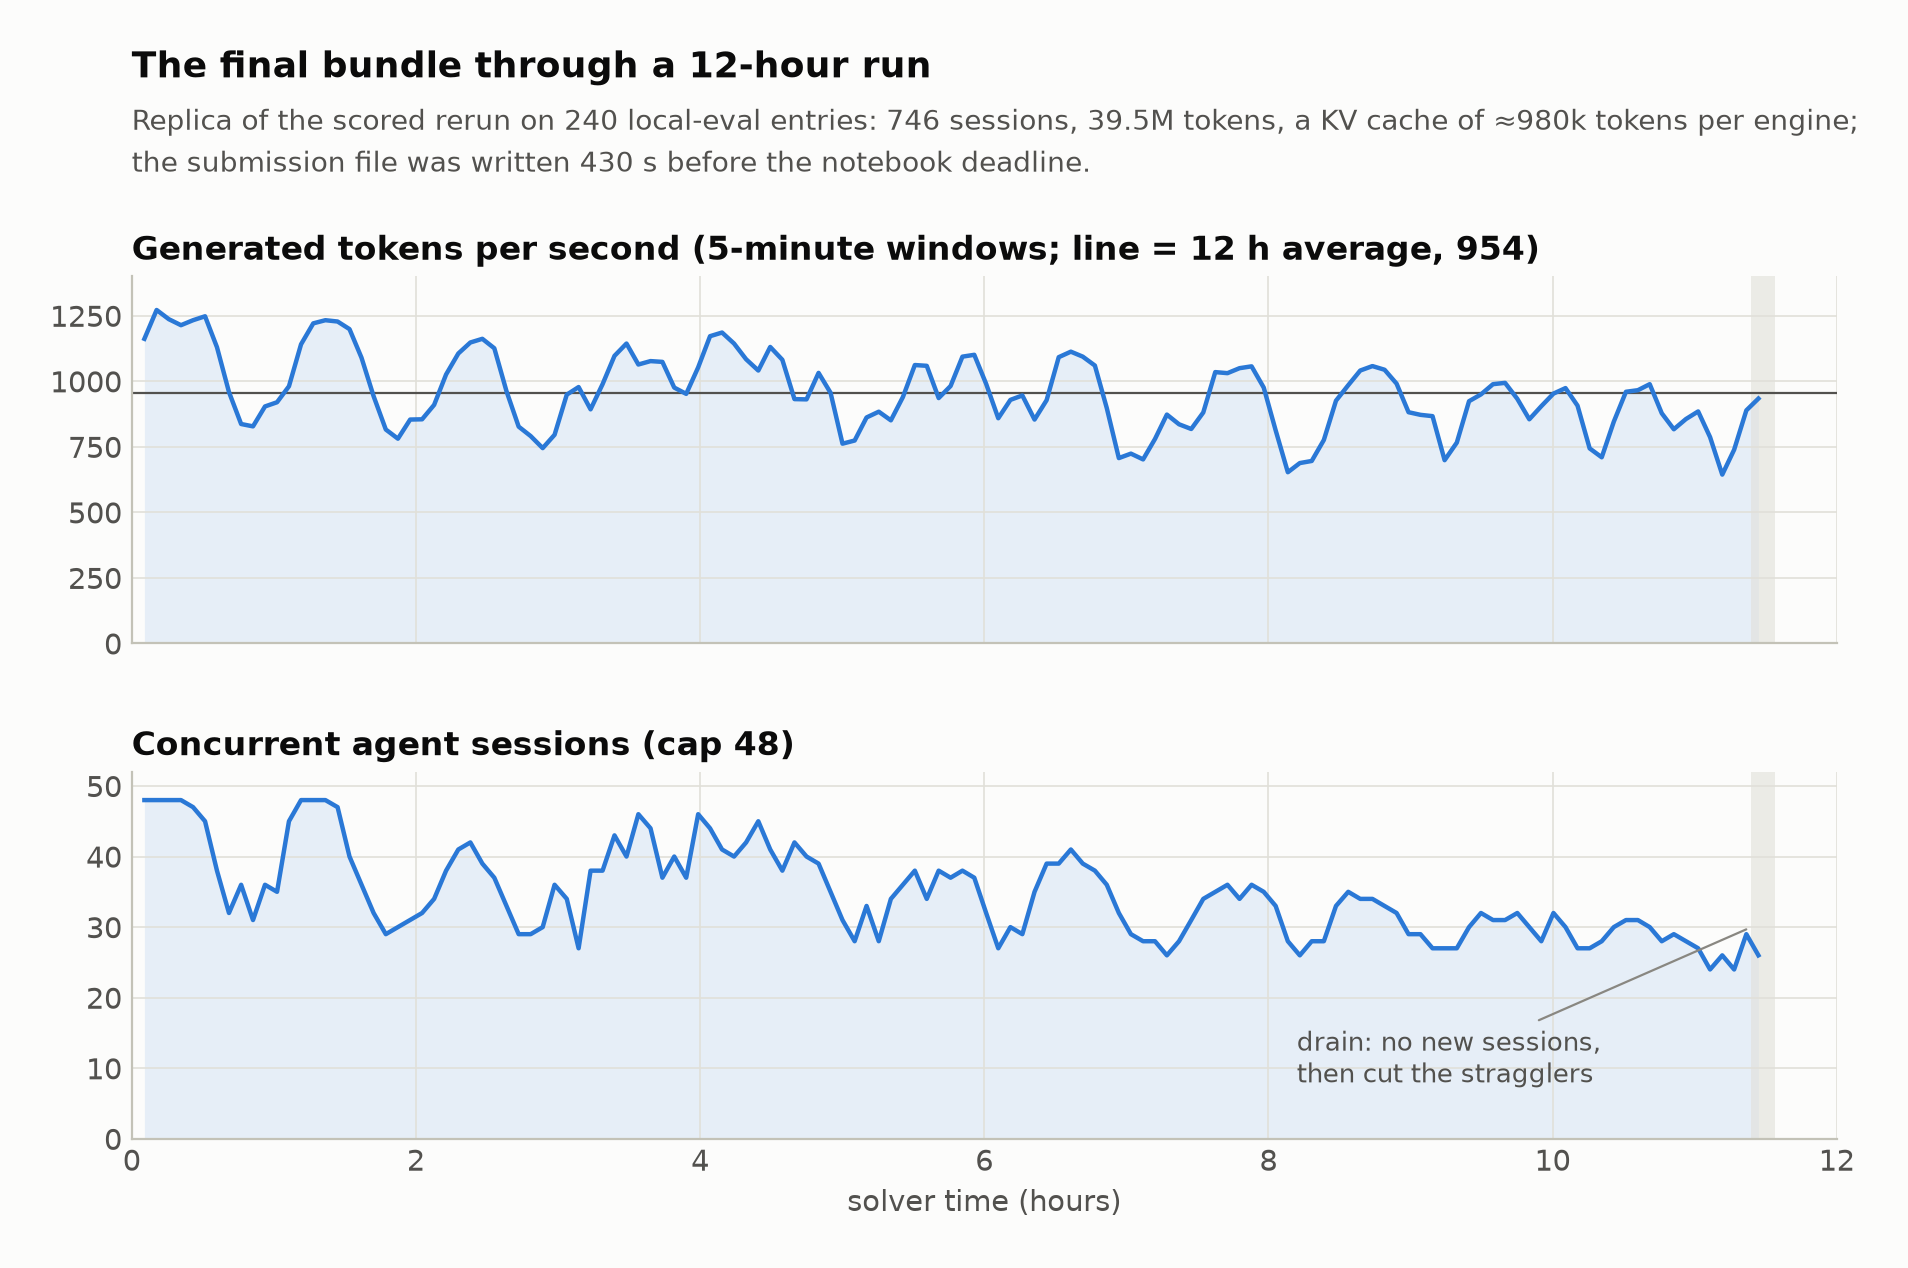
\includegraphics[width=0.94\linewidth]{fig_run_timeline.png}
  \caption{The final bundle through a 12-hour run: tokens/s and concurrent sessions.}
  \label{fig:timeline}
\end{figure}

\paragraph{Scheduling.} At most 2 concurrent sessions per task after its first. Settle-last:
\Dpm{+0.82}{+0.20}{+1.44} in replay. Verified-first \mn3.3, unverified-first \mn1.1, token-fair \mn1.7.

\paragraph{Caps.}
\begin{itemize}
  \item 98,304 generated tokens within a 122,880-token context.
  \item 48k and 32k caps cost 4--5 and 14 points against 80k.
  \item 262k caps added \Dpm{+3.75}{\mn2.5}{+9.4} for 11\% more tokens. Sessions ending above 100k of context are right
        15--16\% of the time but use 39--44\% of tokens.
  \item Tail sessions, sized to the time left (at least 16,384 tokens), produce 17\% of tokens.
\end{itemize}

\paragraph{Admission.} A new session starts only while
\begin{equation*}
  \sum_{i} \max(c_i,\, \tau) + \tau \;\le\; C_{\mathrm{KV}},
  \qquad \tau = \max\big(36\text{k},\ 0.6\,\bar{c}_{50}\big),
\end{equation*}
where $c_i$ is the context of running session $i$, $C_{\mathrm{KV}}$ the KV capacity, and $\bar{c}_{50}$ the mean final
context of the last 50 sessions. Going to 48 sessions added 3--7\% tokens.

\paragraph{Deadline.}
\begin{itemize}
  \item The cut comes 3--10 min before the deadline, set from the measured generation rate. Sessions then stop at their
        next 2,048-token chunk, run any open call and answer.
  \item The submission is rewritten atomically after every session. An input-echo file exists from the first minute,
        and a final cell validates the file and writes an emergency copy.
\end{itemize}

\paragraph{Robustness.}
\begin{itemize}
  \item A length guard ended device asserts that had crashed 5 of 8 full runs.
  \item Capping the recurrent-state fold made session resumes exact.
  \item Reading files in consumption order, plus a compile cache, cut boot from 592\,s to 245\,s.
  \item Supervised server restarts and session retries.
\end{itemize}

\paragraph{Selection.}
\begin{itemize}
  \item Programs verified before 30k tokens have precision 0.80; after 60k, 0.48.
  \item Ranking: votes, the symmetry and test-only-code checks, branch count, then session order; then forced answers
        and partial programs.
  \item \texttt{attempt\_2} fill: +0.22.
  \item Dropped: diverse \texttt{attempt\_2} (\mn0.10 to \mn0.48), two-build ensembles (no better than averaging).
\end{itemize}

% ---------------------------------------------------------------------------------------------------------------
\section{Engine details}\label{app:engine}

\paragraph{Layout.}
\begin{itemize}
  \item Two TP2 engines with 4-way expert parallelism: total KV 1.71M tokens, against 1.17M with TP4.
  \item Full-decode CUDA graphs up to 128 tokens: +5.6\% tokens/s, +10\% KV.
  \item Prefix caching instead of sessions hit only 38\% of the time and cost 11\% KV.
\end{itemize}

\paragraph{Collectives.}
\begin{itemize}
  \item The tensor-parallel all-reduce is one Triton kernel over \texttt{cudaHostRegister}ed shared memory, with
        system-scope flags, fp32 accumulation and 16 thread blocks.
  \item Gathers and scatters use 32\,MB host slots; the logits gather goes through host memory too.
  \item Decode step: 133 $\rightarrow$ 117\,ms.
\end{itemize}

\paragraph{int8.}
\begin{itemize}
  \item Dispatch at 0.516× the bytes.
  \item Reduce-scatter peer shares in int8 per 128-element group, with fp32 scales; the local share stays BF16; only
        above 24 tokens per rank.
  \item KL $1.34$--$1.37\times10^{-2}$, against a floor of $1.27\times10^{-2}$. An int8 all-reduce gained nothing.
\end{itemize}

\paragraph{Kernels.} Together \mn3.7\% per step and +2.6\% KV:
\begin{itemize}
  \item Router before the shared expert, about 0.25\,ms per step.
  \item Concurrent 4/3-bit groups with fused cast-and-add, \mn36 to \mn51\,µs per layer.
  \item L4-tuned Marlin tiles, +2.0\%.
  \item Overlapped Gated DeltaNet projections, about 0.2\,ms per step.
\end{itemize}

\paragraph{Recurrent state.} The fold is deferred into the next verify step: \mn34\% update time.

\paragraph{Memory.}
\begin{itemize}
  \item The n-gram table is 320M rows × 160 FP8 values in one shared-memory file; each rank loads a quarter, and a
        Triton gather runs on a side stream. The 1.18\,GiB token embedding is shared the same way.
  \item FP8 KV for the MTP layer too (BF16 there cost 4.8--7\%).
  \item Recurrent-state groups 6 $\rightarrow$ 4: +6.3\% tokens/s.
  \item Shared top-k: +2.7\% KV.
  \item MoE chunk 2,176: +2.8\% KV.
  \item Allocator and NCCL memory settings: +2--6\% KV.
\end{itemize}

\paragraph{Other.} Batch-sharded sampling: +2.6\%. RC8's flags over RC6's: +7.0\%.

\paragraph{Dropped.} Memory utilization 0.94 (out of memory), placing experts by routed bytes (+0.4\%), batch-token caps
(\mn1.9 to \mn15\%), and five custom kernels that were 1.16--1.46× slower.

\end{document}
